\documentclass{beamer}

\usepackage{beamerthemesplit}
\usetheme{Singapore}

\input{../../include/preamble.inc} 
\input{../../include/definitions.inc} 
\input{../../include/author.inc} 

\title[]{Оператор Гамильтона}

\begin{document}

\frame[plain]{\titlepage}


\frame[plain]{
\frametitle{Аннотация}
\parbox{\textwidth}{
Оператор Гамильтона и его свойства. Дифференциальные операторы первого и второго порядка.
}
}

\frame{
\frametitle{Оператор Гамильтона}
\begin{dfn}
\parbox{\textwidth}{
\alert{Оператором Гамильтона} или \alert{наблой} называется оператор
\[ 
\nabla=\basis{i}\pdx{}+\basis{j}\pdy{}+\basis{k}\pdz{}.
\]
}
\end{dfn}
}

\frame{
\frametitle{Представление дифференциальных операторов через оператор Гамильтона}
\parbox{\textwidth}{
Пусть $\vec{r}=x\basis{i}+y\basis{j}+z\basis{k}$ и заданы
\[
\varphi = \varphi(\vec{r}),\quad
\psi = \psi(\vec{r}),\quad
\vec{a}(\vec{r})=a_x(\vec{r})\basis{i}+a_y(\vec{r})\basis{j}+a_z(\vec{r})\basis{k}
\]
скалярные и векторное поля в $\Rd{3}$. \pause 

\medskip
Тогда дифференциальные операторы с помощью оператора Гамильтона можно записать в виде:
\[
\begin{array}{c}
\grad{\varphi} =  \pause 
\nabla \varphi= \pause 
\pdxds{\varphi}\basis{i}+\pdyds{\varphi}\basis{j}+\pdzds{\varphi}\basis{k},  \\ \pause 
\dv{a} =  \pause 
\nabla \cdot \vec{a} =  \pause 
\dvdefds{a},  \\

\end{array}
\]
}
}


\frame{
\frametitle{Представление ротора через оператор Гамильтона}
\parbox{\textwidth}{

\[ 
\rot{a}= \pause 
\nabla\times\vec{a}= \pause 
\left|\begin{array}{ccc}
\basis{i} & \basis{j} & \basis{k} \\
\pdxds{} & \pdyds{} & \pdzds{} \\
a_x & a_y & a_z 
\end{array}\right|
=
\] \pause 

\bigskip 
\[ 
=
\left(\pdy{a_z}-\pdz{a_y}\right)\basis{i}+
\left(\pdz{a_x}-\pdx{a_z}\right)\basis{j}+
\left(\pdx{a_y}-\pdy{a_x}\right)\basis{k}.
\]



}
}

\frame{
\frametitle{Предварительные замечания}

Пусть $C$ -- константа, тогда
\[
\nabla(C\varphi)= \pause 
\gradv{C\varphi}= \pause 
C\left(\gradv{\varphi}\right)= \pause 
C\nabla\varphi, \pause 
\]

\medskip
\[
\nabla\cdot(C\vec{a})= \pause 
\dvdef{Ca}= \pause 
C\left(\dvdef{a}\right)= \pause 
C\nabla\cdot\vec{a}.
\] \pause 

\medskip
Аналогично
\[
\nabla\times(C\vec{a})=C\nabla\times\vec{a}.
\]
}

\frame{
\frametitle{Предварительные замечания}

Пусть $\vec{c}=c_x\basis{i}+c_y\basis{j}+c_z\basis{k}$ -- постоянный вектор,  \pause тогда
\[
\nabla\cdot (\varphi\vec{c})= \pause 
\dvdef{\varphi c}= \pause 
\left(\gradv{\varphi}\right)\cdot\vec{c}= \pause 
\]
\[
=\vec{c}\cdot\nabla \varphi, \pause 
\] 
\[
\nabla\times(\varphi\vec{c})= \pause 
\left|\begin{array}{ccc}
\basis{i} & \basis{j} & \basis{k} \\
\pdxds{} & \pdyds{} & \pdzds{} \\
\varphi c_x & \varphi c_y & \varphi c_z 
\end{array}\right|= \pause 
\left|\begin{array}{ccc}
\basis{i} & \basis{j} & \basis{k} \\
\pdxds{\varphi} & \pdyds{\varphi} & \pdzds{\varphi} \\
 c_x & c_y & c_z 
\end{array}\right|= \pause 
\nabla\varphi\times\vec{c}.
\]
}


\frame{
\frametitle{Мнемоническое правило для раскрытия производных}

\[ 
\grad{\varphi\psi}= \pause 
\nabla(\varphi\psi)= \pause 
\nabla(\varphi\psi_c)+\nabla(\varphi_c\psi)= \pause 
\psi\nabla\varphi+\varphi\nabla\psi= \pause 
\]
\[
=
\psi\grad{\varphi}+\varphi\grad{\psi}, \pause 
\]
\[ 
\dvwv{\varphi \vec{a}}= \pause 
\nabla\cdot(\varphi\vec{a}) = \pause 
\nabla\cdot(\varphi_c\vec{a}) + \nabla\cdot(\varphi\vec{a}_c) = \pause 
\varphi(\nabla\cdot{a})+\nabla\varphi\cdot\vec{a} = \pause 
\]
\[
=\varphi\dv{a}+\vec{a}\cdot\grad{\varphi}, \pause 
\]
\[ 
\rotwv{\varphi \vec{a}}= \pause 
\nabla\times(\varphi \vec{a})= \pause 
\nabla\times(\varphi_c \vec{a})+\nabla\times(\varphi \vec{a}_c)= \pause 
\varphi(\nabla\times\vec{a})+\nabla\varphi\times \vec{a}= \pause 
\]
\[
=\varphi\rot{a}+\grad{\varphi}\times\vec{a}.
\]


}

\frame{
\frametitle{Дивергенция векторного произведения векторов}
\begin{columns}
\begin{column}{0.3\textwidth}
\centering
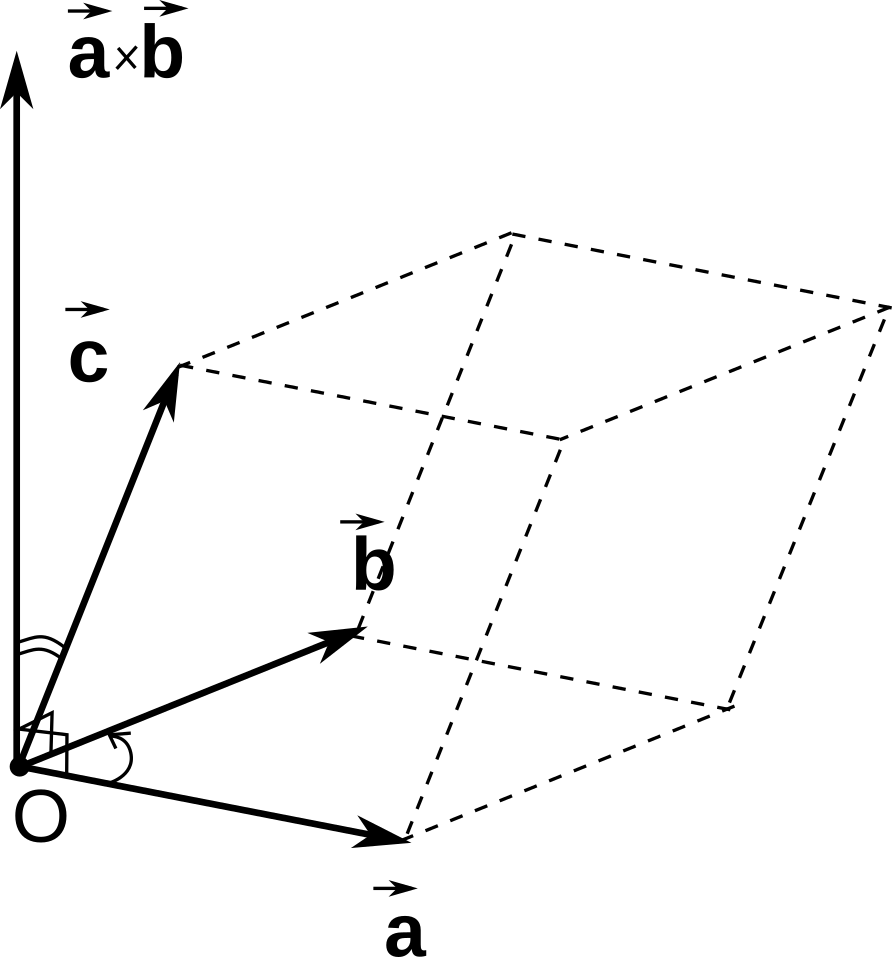
\includegraphics[width=\textwidth]{../img/abc.png}
\end{column}
\begin{column}{0.5\textwidth}
\parbox{\textwidth}{
Объем параллелепипеда, построенного на векторах $\vec{a}$, $\vec{b}$ и $\vec{c}$, равен \pause 
\[
V= \vec{c} \cdot (\vec{a}\times\vec{b})= \pause 
(\vec{c}\times\vec{a})\cdot\vec{b}= \pause 
\]
\[
=(\vec{b}\times\vec{c})\cdot\vec{a}.
\]
}
\end{column}
\end{columns}

\bigskip \pause 
\[
\dvwv{(\vec{a}\times\vec{b})}= \pause 
\nabla\cdot(\vec{a}\times\vec{b})= \pause 
\nabla\cdot(\vec{a}_c\times\vec{b})+\nabla\cdot(\vec{a}\times\vec{b}_c)= \pause 
\]
\[
=-(\nabla\times \vec{b})\cdot\vec{a}+(\nabla\times\vec{a})\cdot\vec{b}= \pause 
\vec{b}\cdot\rot{a}-\vec{a}\cdot\rot{b}.
\]
}

\frame{
\frametitle{Оператор Лапласа}
\parbox{\textwidth}{
\[
\dvwv{\grad{\varphi}}= \pause 
\nabla\cdot\left(\nabla\varphi\right)= \pause 
\left(\gradv{}\right)\cdot\left(\gradv{\varphi}\right)= \pause 
\]
\[
=\lapl{\varphi}=\Delta\varphi
\]
} \pause 

\bigskip
\begin{dfn}
\parbox{\textwidth}{
Оператор 
\[
\Delta=\displaystyle\lapl{}
\]
называется \alert{оператором Лапласа}.
}
\end{dfn}

}

\frame{
\frametitle{Соотношения, полученные ранее}

\[
\dvwv{ \rot{a} } = \nabla\cdot(\nabla\times\vec{a})=0,
\] \pause 
\[
\rotwv{\grad{\varphi}}=\nabla\times(\nabla\varphi)=0,
\] \pause 
\[
\grad{\varphi(r)} = \frac{\varphi'(r)}{r}\vec{r},\quad
r=\sqrt{x^2+y^2+z^2}.
\]

}

\end{document}

